\chapter{Introduction et contexte}
\section{Introduction}
\section{Présentation du laboratoire d'accueil}
Ce stage a eu lieu au Commissariat à l'énergie atomique et aux énergies alternatives (CEA), qui est un acteur majeur de la recherche au service de l'État et des industriels. Le CEA est divisé en quatre directions assurant des missions distinctes telles que la défense et la sécurité nationale (DAM - Direction des Applications Militaires), l'amélioration de la santé publique et l'assistance pour la transition numérique de la société (DRT - Direction de Recherche Technologique), la recherche fondamentale (DRF - Direction de la Recherche Fondamentale) et finalement l'étude des systèmes énergétiques bas-carbone (DES - Direction des Énergies). Ce stage s'est déroulé sur le centre de Cadarache, au Département de Technologie Nucléaire (DTN), appartenant à la Direction des Énergies, au sein du Laboratoire de Modélisation des Accidents Graves (LMAG). Les travaux du laboratoire portent sur le comportement du c\oe ur fondu, que l'on nomme corium, en situation accidentelle. Les principaux axes de recherche du laboratoire sont : l'interaction corium-béton (ICB), l'interaction corium-sodium et le comportement du corium en fond de cuve. Ce laboratoire emploie quinze ingénieurs-chercheurs et quatre doctorants qui travaillent principalement sur la modélisation et la simulation numérique, étant ainsi complémentaire au Laboratoire d'Expérimentation des Accidents Graves (LEAG) qui exploite une plateforme expérimentale (PLINIUS) dédiée au corium prototypique. Le stage a été encadré par Mirantsoa-Aimé Rasolofomanana, doctorant et Romain Le Tellier, ingénieur-chercheur.
\section{Contexte de l'étude}
\subsection{Contexte industriel}
En France, 56 réacteurs nucléaires dispersés sur 18 sites sont actuellement en service, ce parc est uniquement composé de réacteurs à eau pressurisée (REP) et représente 70\% de la production électrique française. Les puissances fournies par ces réacteurs dit de deuxième génération varient entre 900 MWe et 1450 MWe. Un réacteur de troisième génération d'une puissance de 1650 MWe (EPR - European pressurized reactor) est actuellement en construction sur le site de Flamanville, cette nouvelle génération de réacteur tient compte du retour d'expérience issu de l'exploitation des réacteurs actuels, intégrant notamment plus d'éléments de sûreté. La construction de six nouveaux EPR a été annoncée et huit autres pourraient voir le jour. \\
Les REP sont des réacteurs de la famille des réacteurs à eau légère, de l'eau est utilisée comme fluide caloporteur et modérateur, de plus cette eau est pressurisée à 155 bars pour éviter un changement d'état liquide-gaz dans le circuit primaire et ainsi obtenir un meilleur coefficient d'échange thermique, le schéma de principe est présenté par la figure \ref{fig:schcentrale1} %, à l'entrée de la cuve la température de l'eau est 290\textdegree C et la température de sortie de cuve en fonctionnement nominal est de 330\textdegree C.
\begin{figure}[H]
	\centering
	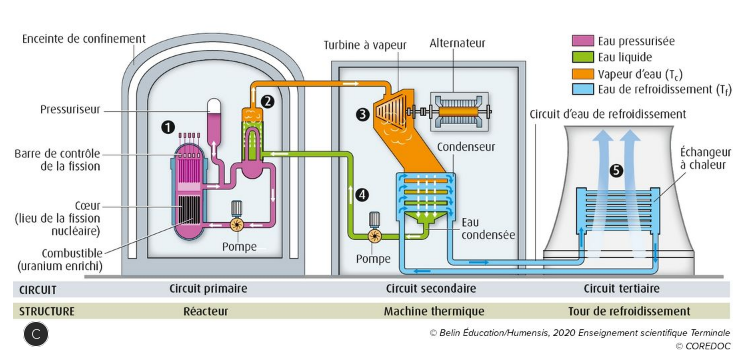
\includegraphics[width=0.8\linewidth]{figure/sch_centrale1}
	\caption[Schéma de principe d'une centrale nucléaire de type REP]{Schéma de principe d'une centrale nucléaire de type REP, (d'après manuelnumeriquemax.belin.education)}
	\label{fig:schcentrale1}
\end{figure} 
\subsection{Généralités sur la sûreté nucléaire}

Les questions de sûreté sont intrinsèquement liées à l'exploitation d'une centrale nucléaire tant les conséquences d'un potentiel accident peuvent être importantes. Ainsi dès le début des années 1970, le concept de défense en profondeur a été mis en place, ce concept se matérialise par la mise en place de lignes de défense successive indépendante. Pour les REP on compte trois barrières de confinement de la radioactivité :
\begin{enumerate}
	\item La gaine combustible
	\item La cuve et l'ensemble du circuit primaire
	\item Le bâtiment réacteur placé sous atmosphère dépressurisée
\end{enumerate}
Les variations par rapport au régime nominal sont classés selon l'échelle INES (International Nuclear Scale Event, figure \ref{fig:echelle-ines-article}), cette échelle permet de classifier les accidents et leurs gravités, elle comporte huit échelons allant d'un simple écart (plusieurs centaines de cas par an en France) à l'accident majeur. Les accidents correspondent aux paliers 4 à 7 et se différencient de l'incident du fait de la perte d'intégrité de la première barrière résultante de la fusion du combustible, le produit de cette fusion est alors appelé corium.
\begin{figure}[H]
	\centering
	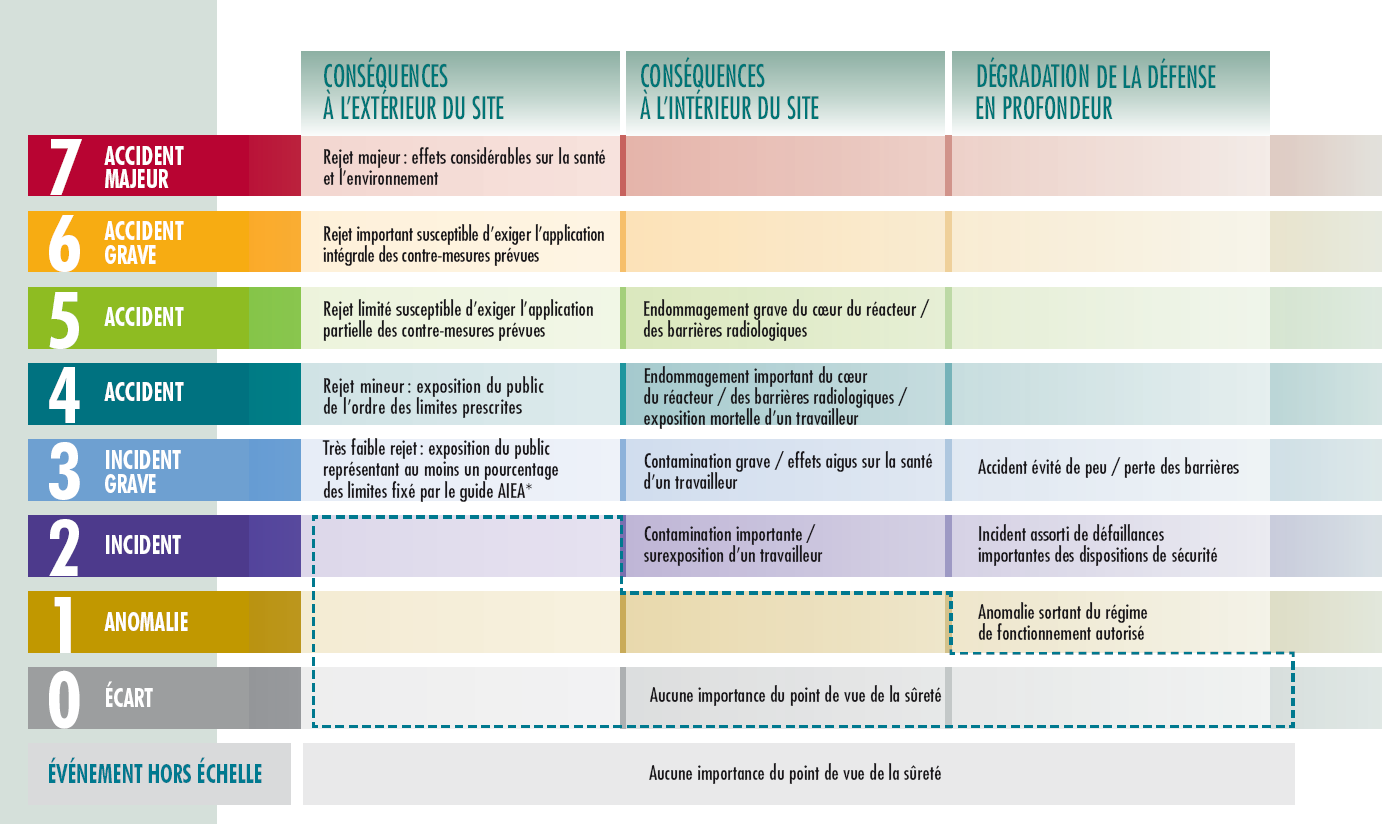
\includegraphics[width=0.7\linewidth]{figure/echelle-ines-article}
	\caption[Echelle de classification des écarts au régime nominal INES]{Echelle de classification des écarts au régime nominal INES (d'après ASN)}
	\label{fig:echelle-ines-article}
\end{figure}
Les accidents possibles dans les REP sont séparés en deux grandes catégories, les accidents de criticité et les Accidents de Perte de Réfrigérant Primaire (APRP). Les accidents de criticité sont dus à une accélération brutale de la réaction en chaîne, le c\oe ur est alors en régime sur-critique entraînant une augmentation rapide de puissance thermique produite, l'accident de Tchernobyl en 1986 est un exemple.\\ Les Accidents de Perte de Réfrigérant Primaire (APRP) résultent quant à eux d'une fuite dans le circuit primaire ou d'un arrêt de la circulation du fluide caloporteur privant le c\oe ur du refroidissement nécessaire à son fonctionnement, un cas d'accident de ce type est Fukushima Daiichi en 2011 où le tsunami à détruit l'alimentation électrique de la centrale, neutralisant ainsi l'ensemble des pompes. Dans la suite de ce rapport nous traiterons uniquement de cette seconde catégorie d'accident.
\subsection{Formation du corium lors d'un accident}
Lors d'un accident de type APRP, l'élévation de la température dans la cuve provoque l'oxydation fortement exothermique des gaines en zircaloy (alliage composé de 98\% de zirconium), cette augmentation de température provoque un ensemble de réactions chimiques décrite en annexe \ref{annexe:seq_deg}. Finalement un bain se forme comprenant de l'uranium, du zirconium et de l'acier ainsi que leurs oxydes respectif, la présence d'une lacune de miscibilité pour la phase liquide du système \{U, O, Zr, Acier\} entraîne une stratification de l'écoulement, ainsi on obtient un écoulement multiphasique et multicomposant. Le corium est un matériau fortement radioactif et produisant sa propre chaleur, l'objectif est alors de maîtriser sa propagation, pour cela deux stratégies existent : la rétention en fond de cuve avec refroidissement externe (explicité plus bas) et l'étalement sur un radier en béton, cette seconde stratégie est préférée pour les réacteurs de puissance élevée comme l'EPR par exemple. L'objectif est d'étaler le corium sur un radier en béton réfractaire, ce béton est alors progressivement ablaté. Pour limiter cette ablation un refroidissement passif est mis en place via le plancher puis une fois le corium partiellement refroidit, celui-ci est recouvert d'eau évitant ainsi une explosion de vapeur.
\subsection{Stratégie de rétention du corium en fond de cuve (IVR)}
Une fois le c\oe ur fondu celui-ci se relocalise au fond de la cuve du réacteur. Pour limiter les conséquences d'un accident une stratégie vise à maintenir ce corium dans le fond de cette cuve, c'est la stratégie d'In-Vessel Retention (IVR). Pour cela on cherche à refroidir la cuve par l'extérieur. Cette stratégie est étudiée depuis les années 90 et mise en \oe uvre sur des réacteurs de faible puissance. \\
Le comportement du corium en fond de cuve est alors régi par deux principaux phénomènes :
La thermohydraulique du bain, avec un écoulement turbulent soumis à des rouleaux de convection (instabilité de Rayleigh-Bénard) dans la phase oxyde, d'autre part la thermochimie régit quant à elle le comportement des phases et leurs équilibres. \\
\subsubsection{Modélisation stationnaire}
Les premières études du comportement du bain de corium ont été réalisés pour des bains stationnaires. Il a été montré qu'en régime stationnaire le bain est stratifié avec une phase oxyde et une phase métal, cependant en fonction de l'accident la couche de métal peut être lourde (i.e plus que l'oxyde et donc être en dessous) ou légère. Les différents cas sont obtenus via des différences de conditions initiales (fraction massique d'acier, degré d'oxydation du zirconium, le rapport molaire entre l'uranium et le zirconium dans la phase oxyde et la température du bain).
\begin{figure}[H]
	\begin{subfigure}[H]{0.47\textwidth}
		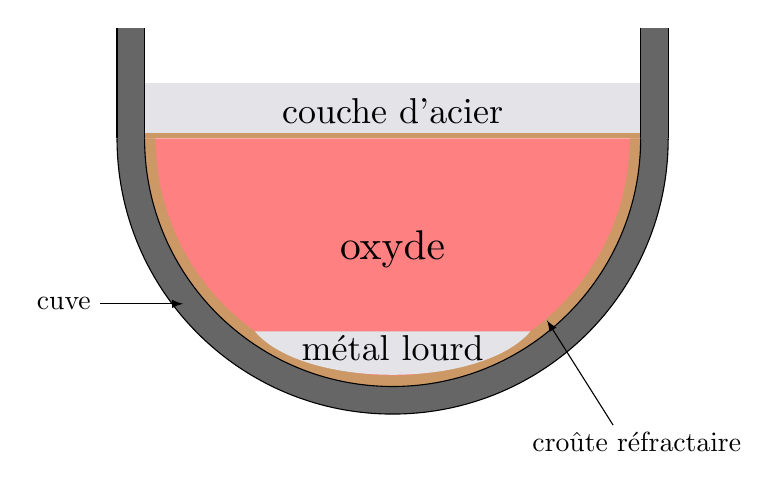
\begin{tikzpicture}[scale=0.70]
		%cuve
		%couche+croute
		\fill[red!50] (0.5,0) arc (180:360:4.5) -- cycle;
		\fill[blue!10!gray!20] rectangle (9.5, 1);
		\fill[brown!80] (0.5,0) arc (180:360:4.5) -- (9.3,0) arc (360:180:4.3) -- cycle;
		\fill[brown!80] rectangle (9.5,0.1);
		\fill[blue!10!gray!20] (2.5,-3.5) ..controls +(0.9,-1.05)and+(-0.9,-1.05) .. (7.5,-3.5) -- cycle ;
		\fill[black!60] (0,2) -- (0,0) arc (180:360:5) -- (10,2) -- (9.5,2) -- (9.5,0) arc (360:180:4.5) -- (0.5,2) -- cycle;
		%cuve
		\draw (0,0) arc (180:360:5);
		\draw (0.5,0) arc (180:360:4.5);
		\draw (0,0) -- (0,2);
		\draw (0.5,0) -- (0.5,2);
		\draw (10,0) -- (10,2);
		\draw (9.5,0) -- (9.5,2);
		
		\draw (5,0.5) node[ scale=1.3]{couche d'acier};
		\draw (5,-2) node[ scale=1.5]{oxyde};
		\draw (5,-3.8) node[ scale=1.3]{métal lourd};
%		
%		\draw[->,>=latex, red, line width = 2mm] (1.3, 0.5) to (0.1, 0.5);
%		\draw[->,>=latex, red, line width = 2mm] (8.7, 0.5) to (9.9, 0.5);
		
		%FE
%		\draw[black, dashed, thick] (3.2,0.2) circle (0.8);
		%\draw[black, dashed, thick] (9.3,0.5) circle (0.8);
%		\draw[->,>=latex] (0.5, 0.8) to (4, 2);
%		\draw[->,>=latex] (9.3, 0.8) to (6, 2);
%		\draw (5,2.3) node[ scale=1.3]{Focusing Effect};
		
		%cuve
		\draw[->,>=latex] (-0.3, -3) to (1.2, -3);
		\draw (-0.3, -3) node[ scale=1, left]{cuve};
		
		%croute
		
		\draw[->,>=latex] (9, -5.2) to (7.8, -3.3);
		%\draw (1, -4.2) -- (-0.3, -4.2);
		\draw (11.5, -5.5) node[ scale=1, left]{croûte réfractaire};
		
		%echange
		%\draw[->,>=latex,line width = 0.8mm] (3.2, -0.6) to (3.2, -3.8);
		
		
%		\draw[->,>=latex,line width = 0.5mm] (2.8, 0.8) to (2.8, -1.2);
%		\draw (2.2,0.7) node[ scale=1]{(Fe)};
%		\draw[->,>=latex,line width = 0.5mm](3.5, -1.2) to (3.5, 0.8);
%		\draw (4.2,-1) node[ scale=1]{(U,Zr)};
		%\draw (2,0.5) node[ scale=1]{(Fe)};
		%\draw[->,>=latex,line width = 0.5mm](2.7, -1.2) to (2.7, 0.8);
		%\draw (3.4,-1) node[ scale=1]{(U,Zr)};
		%\draw[blue, very thick] (7.3, 0.1) -- (7.3, 1);
		%\draw[blue, thick] (7.2, 0.1) -- (7.4, 0.1);
		%\draw[blue, thick] (7.2, 1) -- (7.4, 1);
		%\draw (7.3, 0.5) node[ scale=1.3, right, blue]{$H$};
		\end{tikzpicture}
			\caption{Première configuration}
			\label{fig:confmetallourd}
	\end{subfigure}
	\hfil
	\begin{subfigure}[H]{0.47\textwidth}
	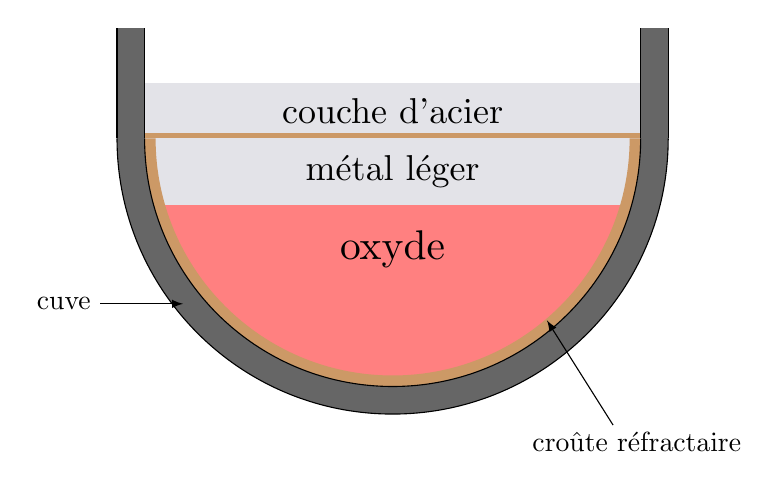
\begin{tikzpicture}[scale=0.70]
	%cuve
	%couche+croute
	\fill[red!50] (0.5,0) arc (180:360:4.5) -- cycle;
	\fill[blue!10!gray!20] rectangle (9.5, 1);
	\fill[brown!80] rectangle (9.5,0.1);
	\fill[blue!10!gray!20] (0.5,0) rectangle (9.5, -1.2);
%	\fill[blue!10!gray!20] (2.5,-3.5) ..controls +(0.9,-1.05)and+(-0.9,-1.05) .. (7.5,-3.5) -- cycle ;
	\fill[black!60] (0,2) -- (0,0) arc (180:360:5) -- (10,2) -- (9.5,2) -- (9.5,0) arc (360:180:4.5) -- (0.5,2) -- cycle;
	\fill[brown!80] (0.5,0) arc (180:360:4.5) -- (9.3,0) arc (360:180:4.3) -- cycle;
	%cuve
	\draw (0,0) arc (180:360:5);
	\draw (0.5,0) arc (180:360:4.5);
	\draw (0,0) -- (0,2);
	\draw (0.5,0) -- (0.5,2);
	\draw (10,0) -- (10,2);
	\draw (9.5,0) -- (9.5,2);
	
	\draw (5,0.5) node[ scale=1.3]{couche d'acier};
	\draw (5,-0.6) node[ scale=1.3]{métal léger};
	\draw (5,-2) node[ scale=1.5]{oxyde};
%	\draw (5,-3.8) node[ scale=1.3]{métal lourd};
	%		
	%		\draw[->,>=latex, red, line width = 2mm] (1.3, 0.5) to (0.1, 0.5);
	%		\draw[->,>=latex, red, line width = 2mm] (8.7, 0.5) to (9.9, 0.5);
	
	%FE
	%		\draw[black, dashed, thick] (3.2,0.2) circle (0.8);
	%\draw[black, dashed, thick] (9.3,0.5) circle (0.8);
	%		\draw[->,>=latex] (0.5, 0.8) to (4, 2);
	%		\draw[->,>=latex] (9.3, 0.8) to (6, 2);
	%		\draw (5,2.3) node[ scale=1.3]{Focusing Effect};
	
	%cuve
	\draw[->,>=latex] (-0.3, -3) to (1.2, -3);
	\draw (-0.3, -3) node[ scale=1, left]{cuve};
	
	%croute
	
		\draw[->,>=latex] (9, -5.2) to (7.8, -3.3);
%\draw (1, -4.2) -- (-0.3, -4.2);
\draw (11.5, -5.5) node[ scale=1, left]{croûte réfractaire};
	
	%echange
	%\draw[->,>=latex,line width = 0.8mm] (3.2, -0.6) to (3.2, -3.8);
	
	
	%		\draw[->,>=latex,line width = 0.5mm] (2.8, 0.8) to (2.8, -1.2);
	%		\draw (2.2,0.7) node[ scale=1]{(Fe)};
	%		\draw[->,>=latex,line width = 0.5mm](3.5, -1.2) to (3.5, 0.8);
	%		\draw (4.2,-1) node[ scale=1]{(U,Zr)};
	%\draw (2,0.5) node[ scale=1]{(Fe)};
	%\draw[->,>=latex,line width = 0.5mm](2.7, -1.2) to (2.7, 0.8);
	%\draw (3.4,-1) node[ scale=1]{(U,Zr)};
	%\draw[blue, very thick] (7.3, 0.1) -- (7.3, 1);
	%\draw[blue, thick] (7.2, 0.1) -- (7.4, 0.1);
	%\draw[blue, thick] (7.2, 1) -- (7.4, 1);
	%\draw (7.3, 0.5) node[ scale=1.3, right, blue]{$H$};
	\end{tikzpicture}
	\caption{Seconde configuration}
\end{subfigure}
\caption{Présentation des différents régimes de stratification possible}
\end{figure}
L'objectif de la rétention en cuve est alors de maintenir ce bain jusqu’à sa solidification, le refroidissement est assuré par convection naturelle sur la paroi de la cuve et par rayonnement sur la face supérieur de la couche d'acier. Cependant la couche supérieure d'acier étant très conductrice et ayant un contact direct avec la cuve sur une surface très faible (la couche d'acier est haute de quelques dizaines de centimètres), la densité de flux transmise est très importante. Cet effet est appelé \textit{"focusing effect"} et représente la principale menace pour l'intégrité de la cuve.
\subsubsection{Modélisation du régime transitoire}
Comme expliqué précédemment, c'est au contact entre la cuve et la couche d'acier que le risque de percement est le plus important. Des études plus récentes ont montré que l'épaisseur de la couche d'acier pouvait être plus fine en régime transitoire qu'en régime stationnaire, diminuant ainsi la surface de contact et aggravant le \textit{"focusing effect"}, c'est pourquoi une modélisation du régime transitoire est désormais préférée. Lors du transitoire des phénomènes d'inversion de phase sont observés, une partie du métal de la phase légère s'alourdit sous l'effet d'un transfert de masse et des gouttes tombent, puis sous l'effet d'un même transfert de masse la phase lourde remonte. On observe alors trois couches : une couche d'oxyde, une de métal léger localiser au dessus de la couche d'oxyde et une couche de métal lourd en fond de cuve ainsi, croûte réfractaire située entre les phases liquides et la cuve est également présente. Finalement on se retrouve dans la situation suivante :
\begin{figure}[H]
	\centering
	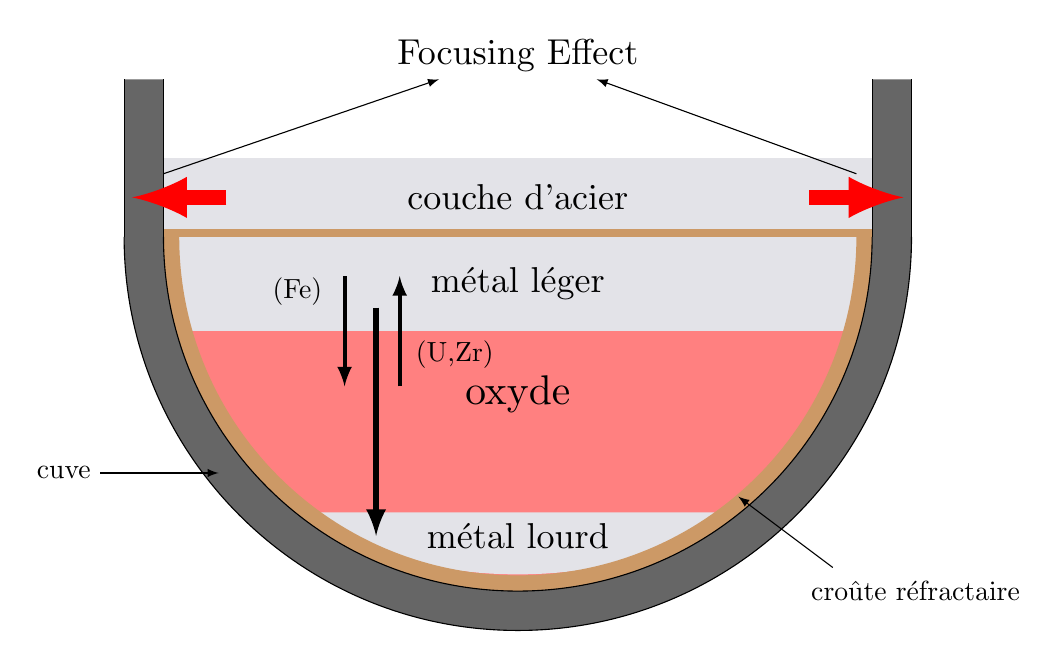
\begin{tikzpicture}
	

	
	%couche+croute
	\fill[red!50] (0.5,0) arc (180:360:4.5) -- cycle;
	\fill[blue!10!gray!20] (0.5,0) rectangle (9.5, 1);
	
	\fill[brown!80](0.5,0) rectangle (9.5,0.1);
	\fill[blue!10!gray!20] (0.5,0) rectangle (9.5, -1.2);
	\fill[blue!10!gray!20] (2.5,-3.5) ..controls +(0.9,-1.05)and+(-0.9,-1.05) .. (7.5,-3.5) -- cycle ;
	\fill[brown!80] (0.5,0) arc (180:360:4.5) -- (9.3,0) arc (360:180:4.3) -- cycle;
	%cuve
	\fill[black!60] (0,2) -- (0,0) arc (180:360:5) -- (10,2) -- (9.5,2) -- (9.5,0) arc (360:180:4.5) -- (0.5,2) -- cycle;
	%cuve
	\draw (0,0) arc (180:360:5);
	\draw (0.5,0) arc (180:360:4.5);
	\draw (0,0) -- (0,2);
	\draw (0.5,0) -- (0.5,2);
	\draw (10,0) -- (10,2);
	\draw (9.5,0) -- (9.5,2);
	
	\draw (5,0.5) node[ scale=1.3]{couche d'acier};
	\draw (5,-2) node[ scale=1.5]{oxyde};
	\draw (5,-3.8) node[ scale=1.3]{métal lourd};
	\draw (5,-0.6) node[ scale=1.3]{métal léger};
	
	\draw[->,>=latex, red, line width = 2mm] (1.3, 0.5) to (0.1, 0.5);
	\draw[->,>=latex, red, line width = 2mm] (8.7, 0.5) to (9.9, 0.5);
	
	%FE
	%\draw[black, dashed, thick] (3.2,-1) circle (0.5);
	%\draw[black, dashed, thick] (9.3,0.5) circle (0.8);
	\draw[->,>=latex] (0.5, 0.8) to (4, 2);
	\draw[->,>=latex] (9.3, 0.8) to (6, 2);
	\draw (5,2.3) node[ scale=1.3]{Focusing Effect};
	
	%cuve
	\draw[->,>=latex] (-0.3, -3) to (1.2, -3);
	\draw (-0.3, -3) node[ scale=1, left]{cuve};
	
	%croute
	
	\draw[->,>=latex] (9, -4.2) to (7.8, -3.3);
	%\draw (1, -4.2) -- (-0.3, -4.2);
	\draw (11.5, -4.5) node[ scale=1, left]{croûte réfractaire};
	
	%echange
	\draw[->,>=latex,line width = 0.8mm] (3.2, -0.9) to (3.2, -3.8);
	
	
	\draw[->,>=latex,line width = 0.5mm] (2.8, -0.5) to (2.8, -1.9);
	\draw (2.2,-0.7) node[ scale=1]{(Fe)};
	\draw[->,>=latex,line width = 0.5mm](3.5, -1.9) to (3.5, -0.5);
	\draw (4.2,-1.5) node[ scale=1]{(U,Zr)};
	%\draw (2,0.5) node[ scale=1]{(Fe)};
	%\draw[->,>=latex,line width = 0.5mm](2.7, -1.2) to (2.7, 0.8);
	%\draw (3.4,-1) node[ scale=1]{(U,Zr)};
	%\draw[blue, very thick] (7.3, 0.1) -- (7.3, 1);
	%\draw[blue, thick] (7.2, 0.1) -- (7.4, 0.1);
	%\draw[blue, thick] (7.2, 1) -- (7.4, 1);
	%\draw (7.3, 0.5) node[ scale=1.3, right, blue]{$H$};
	\end{tikzpicture}
	\caption[]{Schéma du comportement du corium en fond de cuve en régime transitoire, d'après \cite{rasolofomanana_modelisation_nodate}}
	\label{fig:ivrschema}
\end{figure}
La couche de métal lourd se forme à partir d'un transfert de masse a l'interface des phases oxyde et métal léger créant des gouttes d'acier lourd se relocalisant en fond de cuve. L'essai expérimental MASCA RCW, au cours duquel 45kg de corium ont été mis en contact avec 4kg d'acier de telle sorte que le régime stationnaire soit caractérisé par la présence d'une phase métal lourd (configuration de la figure \ref{fig:confmetallourd}), cependant la remontée de la phase lourde vers la phase légère n'a jamais été observée, l'essai ayant été arrêté au bout de 20 minutes le régime stationnaire n'a pas été atteint. Le résultat de cet essai est présenté en figure \ref{fig:masca}, on y observe la présence des gouttes de métal et les différentes phase (la largeur des lingots est d'environ 7cm).
 \begin{figure}[H]
	\centering
	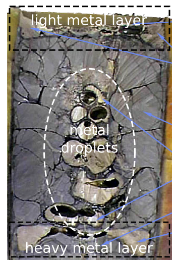
\includegraphics[width=0.3\linewidth]{figure/MASCA_RCW.png}
	\caption[Résultat MASCA-RCW 100]{Résultat MASCA-RCW 100 ,d'après \cite{tellier_interfaces_2019}}
	\label{fig:masca}
\end{figure}


\section{Objectif du stage}
L'objectif du stage est de réaliser une validation qualitative du code CFD (\textit{Computional Fluid Dynamic}) implémenté dans TrioCFD, code Open-Source du CEA, par M.A Rasolofomanana lors de sa thèse \cite{rasolofomanana_modelisation_nodate}. Ce code est une généralisation de la méthode champ de phase pour un système multicomposant. Cette implémentation fait suite aux thèses de Clément Cardon \cite{cardon_modelisation_2016} et de Vaishnvi Tiwari \cite{tiwari_consistent_2019} sur la modélisation par la méthode de champ de phase pour un système multicomposant. L'expérience reproduite est présentée dans \cite{rao_influence_2015}, on y trouve une goutte qui sous l'effet d'un transfert de masse va subir une inversion de densité. Cette validation nécessite une paramétrisation cohérente du système pour obtenir des simulations consistante vis-a-vis d'un système binaire et du comportement thermodynamique. Le développement de ce type de code CFD a pour but de permettre la vérification et l'amélioration des lois de fermetures présente dans des codes intégraux, comme par exemple PROCOR développé au laboratoire.